\documentclass[a4paper,12pt]{article}
\usepackage{times}
\usepackage[francais]{babel}
\usepackage[utf8]{inputenc}
\usepackage[T1]{fontenc}
\usepackage{amsmath}
\usepackage{amssymb}
\usepackage{graphicx}
\usepackage{pdfpages}
\usepackage{pdflscape}
\usepackage{listings}
\usepackage{longtable}
\usepackage{hyperref}
\lstset{literate=
{é}{{\'e}}1
{è}{{\`e}}1
{ê}{{\^e}}1
{à}{{\`a}}1
{â}{{\^a}}1
}
\lstset{language=C++,
                basicstyle=\footnotesize,
                keywordstyle=\footnotesize\color{blue},
                otherkeywords={override,nullptr}
}
\definecolor{orange}{rgb}{0.8,0.4,0.0}
\definecolor{darkblue}{rgb}{0.0,0.0,0.6}
\definecolor{cyan}{rgb}{0.0,0.6,0.6}
\lstdefinelanguage{JSON}
{
  basicstyle=\normalsize,
  columns=fullflexible,
  showstringspaces=false,
  commentstyle=\color{gray}\upshape,
  morestring=[b]",
  morestring=[s]{>}{<},
  morecomment=[s]{<?}{?>},
  stringstyle=\color{orange},
  identifierstyle=\color{darkblue},
  keywordstyle=\color{blue},
  morekeywords={string,number,array,object}% list your attributes here
}

\sloppy

\setlength{\topmargin}{0cm}
\setlength{\headsep}{0.in}
\setlength{\headheight}{0.in}
\setlength{\evensidemargin}{0cm}
\setlength{\oddsidemargin}{-1cm}
\textwidth 18cm
\textheight 25cm

\begin{document}

\thispagestyle{empty}

\begin{titlepage}

\vspace*{2cm}

\begin{center}\textbf{\Huge Projet Logiciel Transversal}\end{center}{\Large \par}

\begin{center}\textbf{\large Alexandre Génot - Anthony Peloille}\end{center}{\large \par}

\vspace{2cm}

\begin{figure}[h]
\begin{center}

\includegraphics[width=\textwidth]{thelegendofzelda.png}
\caption{\label{The Legend of Zelda}The Legend of Zelda (1986)}
\end{center}
\end{figure}

\clearpage

{\small
\tableofcontents
}

\end{titlepage}

\clearpage
\section{Présentation Générale}

\subsection{Archétype}

Les mécaniques du jeu s'inspirent de The Legend of Zelda (1986) qui est un jeu de type action/aventure.

\subsection{Règles du jeu}

Le joueur évolue dans un donjon avec plusieurs étages. A chaque étage il doit atteindre un boss, pour cela il se déplace de case en case à la manière d’un jeu de plateau. Les cases peuvent contenir différents types d'évènements : combat, récompense, bonus, malus.... Le but est de sortir du donjon en ayant complété chaque étage, c'est-à-dire avoir vaincu chacun des boss. 
\bigbreak
Les phases de combats se déroulent sous forme de combats au tour par tour, à chaque tour le personnage peut attaquer (différents coups d'épée) puis le tour suivant, l'ennemi attaque. Chaque personnage (personnage principal ou ennemi) dispose de 3 caractéristiques :
- Les points de vie/Health Points, lorsque ceux-ci arrivent à 0 le personnage meurt. 
- L'attaque , conditionne les dégâts qu'inflige un coup.
- La défense, détermine la quantité de point de vie perdue après avoir reçu une attaque.
\bigbreak
 Le personnage peut, au cours de son aventure, augmenter ses statistiques.

\subsection{Ressources}

\begin{figure}[h]
\begin{center}
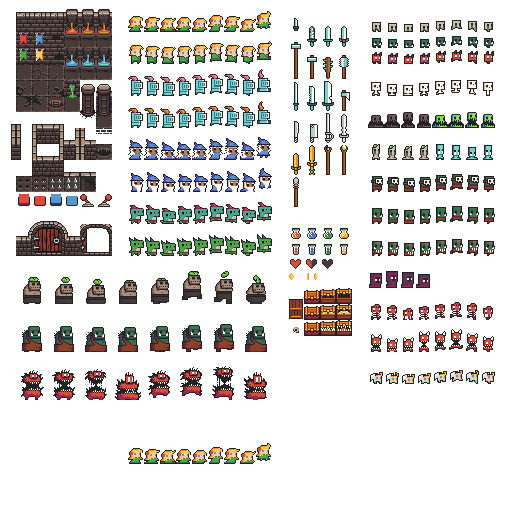
\includegraphics[width=0.5\textwidth]{dungeontiles.png}
\caption{\label{tiles}Tuiles du décor et personnages}
\end{center}
\end{figure}

\begin{figure}[h]
\begin{center}
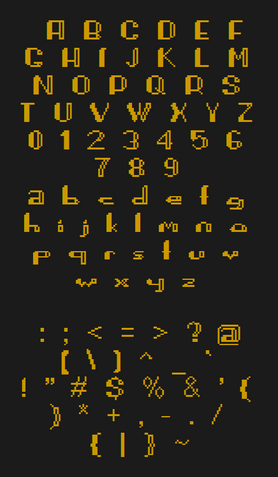
\includegraphics[width=0.5\textwidth]{font.png}
\caption{\label{font}Police de caractères}
\end{center}
\end{figure}

\clearpage
\section{Description et conception des états}

\subsection{Description des états}

Pour chacun des états du jeu, on retrouve une combinaison d'éléments fixes (la structure du labyrinthe) et d'éléments mobiles (personnage principal et ennemis).
Seuls les personnages mobiles possèdent une position sous forme de coordonnées (x et y). Pour les éléments statiques, nous initialisons un tableau avec des éléments.
Tous les éléments ont en commun un identifiant qu'est le TypeId (un id pour les murs, un pour les ennemis, le personnage principal ...).

\subsubsection{État éléments fixes}

Chaque étage du donjon possède un certain nombre fixe de cases. Toutes les cases ont un type parmi ces 4 : Mur, Espace (vide), Porte, Coffre.
\bigbreak
Cases "Mur" (Wall) : Elles servent à délimiter les contours de chaque étage du donjon, les personnages ne pouvant pas les traverser.
\bigbreak
Cases "Espace" (Space) : Il s'agit des cases sur lesquelles peuvent se déplacer librement les éléments mobiles, on trouve plusieurs sous-types de cases Espace :
- Une case de départ où apparaît le joueur.
- Une case de fin qui permet au joueur de passer à l'étage suivant (située après le boss de l'étage).
- Plusieurs cases "spawn" où apparaissent les ennemis.
- Des cases vides de tout élément.
\bigbreak
Cases "Porte" (Door) : Ce sont des cases infranchissables par le joueur sauf si le joueur remplit les conditions requises (avoir tué un certain ennemi, avoir obtenu une clé ...), la case devient alors franchissable et donne accès à une nouvelle zone.
\bigbreak
Cases "Coffre" (Chest) : Ce dernier type de case correspond à des cases qui permettent au joueur d'obtenir des éléments lui permettant de booster ses statistiques (Vitalité, Attaque ou Défense).

\subsubsection{État éléments mobiles}

Les éléments mobiles ont 3 caractéristiques, une direction (les 4 points cardinaux et une direction nulle), une position et une variable (isFighting) indiquant si l'élément est en combat ou non.
Lorsque la position est à 0 alors l'élément est exactement sur la case, sinon il se trouve entre sa case originale et la case qui correspond à sa direction, quand la position à la même valeur que la vitesse, le personnage se déplace dans la direction correspondante.
\bigbreak
Nous avons défini 2 éléments mobiles que sont les ennemis (2 types pour le moment : Ghost, l'ennemi basique et Boss, l'ennemi plus puissant qui permet d'accéder à l'étage suivant) et le personnage principal (MainCharacter) qui n'est autre que le personnage contrôlé par le joueur.
Ces éléments mobiles démarrent avec un certain nombre de PV (exemple 6 pv pour le joueur), si leurs points de vie atteignent 0, pour les ennemis, ils disparaissent du jeu et pour le joueur, cela signifie la fin de la partie.
Comme détaillé dans la partie règle du jeu, ces éléments disposent de 3 caractéristiques sui déterminent leurs puissances de combat (HealthPoints, Attack et Defense).

\subsubsection{État général}

On rajoute enfin 2 éléments généraux à ceux définis auparavant, il s'agit des variables epoch et epochRate.
La première sert simplement à connaître le nombre de "tour" depuis le début de la partie. 
La seconde permet de régler la vitesse du jeu en réglant le nombre d'époque par seconde.

\subsection{Conception Logiciel}

On peut voir notre diagramme des classes sur la page suivante (Figure 4), on y retrouve donc toutes les classes mentionnées auparavant qui permettent de définir un état du jeu :
- MobileElement qui permet de définir des éléments mobiles et dont héritent les classes Monstre (ennemis) et MainCharacter (personnage jouable).
- StaticElement qui à le même rôle pour les éléments statiques qu'on retrouvera dans les étages de notre donjon : murs, portes, coffres ou "sol" permettant aux personnages de se déplacer.
- State qui gère la vitesse du jeu et le nombre de tours effectués.
- Il y aussi de nombreuses classes dédiées à l'énumération de statuts ou de types.
\bigbreak
Il reste donc 3 classes : 
\bigbreak
Classe Element : Cette classe permet de définir chacun des éléments du jeu, qu'ils soient statiques ou mobiles. Elle contenait à l'origine les coordonnées (x,y) de chaque élément mais ceux-ci n'étaient utiles que pour les éléments mobiles. Nous avons tout de même gardé la classe element pour sa liaison avec TypeId et pour éviter de changer une grande partie des fonctions déjà implémentés.
\bigbreak
Classe ElementTab :  Comme son nom le laisse entendre, on a ici, un conteneur d'éléments qui n'est autre qu'un tableau en deux dimensions. Celui-ci contient donc l'intégralité des éléments dispersés sur un étage du donjon.
Son format est un vecteur de vecteur (donc un tableau) de unique ptr, ce format nous a paru pratique puisque nous n'avons pas à préciser la taille dès la définition de l'attribut et le unique ptr nous permet de facilement accéder à chacun des éléments dans le tableau.
A noter que le conteneur principal est la classe State qui contient la totalité des données liées à un état donné.
\bigbreak
Classe Observable : Le but de cette classe va être de réagir à des modifications de l'état du jeu (donc de la classe state), cette classe s'avère surtout utile pour les éléments de rendus qui mettront à jour les sprites. On a 2 types d'événements : TabEvent et StateEvent qui héritent de la classe Event.

StateEvent correspond aux événements qui touchent ce qu'on trouvera dans la classe StateLayer, c'est-à-dire le personnage principal, les monstres, les éléments annexes affichés (boutons, vitalité du perso, texte ...).

TabEvent correspond de son côté aux éléments contenus dans les tableaux ElementTab, donc les sols, murs, coffres ou portes (il y aura notamment des event liés à l'ouverture d'un coffre ou d'une porte).
\bigbreak
Il est à noter qu'afin de pouvoir fabriquer des nouvelles instances d'éléments, nous avons décidé d'implémenter une méthode clone() pour chacun des éléments (statiques ou mobiles) que nous pouvons construire. 
L'implémentation de cette méthode répond à un problème lié au format de notre tableau d'élément (vector(vector(unique ptr(Element)))), lorsque nous souhaitons ajouter un élément au tableau, l'élément doit être cloné avant d'être ajouté au tableau sinon celui-ci est doublement détruit (double free).

\begin{landscape}
\begin{figure}[p]
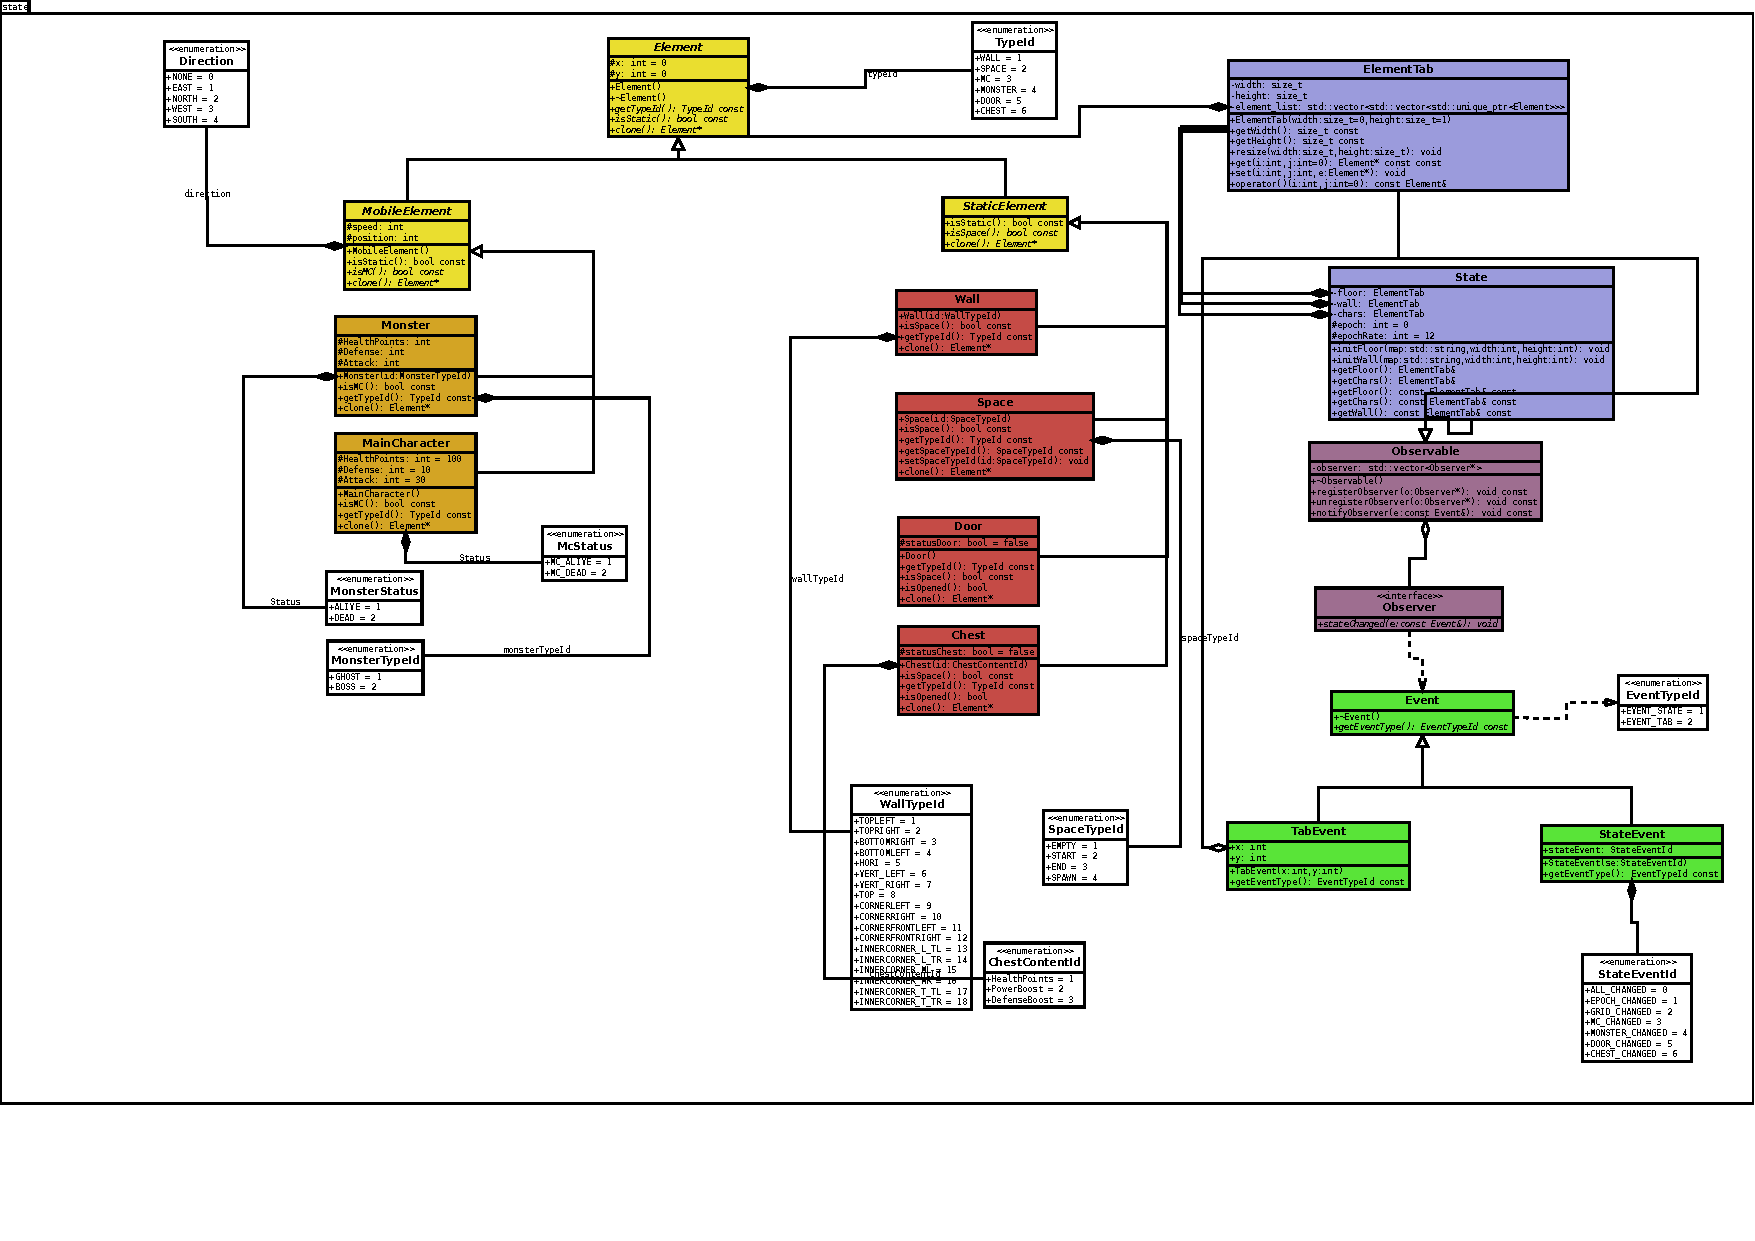
\includegraphics[width=0.9\paperheight]{state.pdf}
\caption{\label{uml:state}Diagramme des classes d'état.} 
\end{figure}
\end{landscape}

\clearpage

\section{Rendu: Stratégie et Conception}

\subsection{Stratégie de rendu d'un état}

Pour la stratégie de rendu d'un état, nous avons choisi de diviser les éléments que nous affichons à l'écran en plusieurs plans/layers.
\bigbreak
Le premier plan nommé floorLayer contient le sol, il recouvre la totalité de la map avec des éléments de type Floor.
Le second plan nommé wallLayer contient les autres éléments statiques : mur, coffres ou portes.
Enfin, il reste un dernier plan stateLayer qui sert à afficher les personnages (personnage principal ou monstre ) contenus dans des listes et non des tableaux car ils possèdent des coordonnées en argument, ce plan sert aussi à afficher des éléments secondaires comme une barre de vie, du texte, des boutons pour le déplacement ou l'attaque ...
\bigbreak
Pour créer notre map, nous utilisons des fichiers .txt contenus dans le dossier src (donc pas à la racine du projet), pour l'instant nous avons écrit 2 fichiers txt, un par layer que nous avons crée (Floor et Wall), à noter que le fichier wall.txt contient des informations sur tous les éléments affichés à l'écran autres que le sol.
Nous avons affecté à chacune des tuiles un ID qui se lit de la manière suivante :
- Le premier chiffre correspond au TypeID de l'objet (1 = wall, 2 = space ...).
- Le second (peut être supérieur à 10) correspond au sous-type d'élément, par exemple si c'est un mur de type vertical, on a le WallTypeID vert = 6 (on écrira alors 16 dans le fichier txt). Si c'est un élément space "vide" on a le SpaceTypeID empty = 1 (on écrira cette fois-ci 21 dans le fichier txt).
Ces fichiers texte sont lus dans les fonctions initWall et initFloor de la classe State, ces méthodes initialise des tableaux d'éléments à partir du contenu de ces fichiers avant de les transmettre aux classes utilisées pour le rendu.


\subsection{Conception logiciel}

Le diagramme des classes pour notre rendu est visible sur la page suivante.
\bigbreak
ElementTabLayer et State Layer : Il s'agit des 2 classes héritant de la classe Layer et permettant de définir les plans que nous allons afficher, les valeurs contenus dans ces tableaux sont définis auparavant dans la classe State.
Ces informations sont données à une instance de Surface et la définition des tuiles est contenue dans une instance de TileSet.
La méthode InitSurface() fait la plus grosse partie du travail : elle fabrique une nouvelle surface puis initialise le nombre de quads/sprites avec la méthode InitQuads() avant de fixer une tuile et une position pour chacun des sprites avec la méthode setSprite().
\bigbreak
Surfaces : Chaque surface contient une texture du plan et un nombre de quadruplets de vecteurs 2D. Les éléments texCoords de chacun des quadruplets contient les coordonnées de 4 coins de la tuile à sélectionner dans la texture. Les éléments position de chaque quadruplet contiennent les coordonnées des quatre coins du carré où doit être dessiné la tuile à l'écran.
\bigbreak
Tuiles : Les classes intéressantes sont les classes filles de la classe TileSet, ces classes contiennent des listes contenant toutes les tuiles d'un certain élément à afficher, par exemple, la liste walls de GridTileSet contient une liste des tuiles correspondant à tous les différents types de murs (coin en haut à gauche, à droite, mur horizontal, vertical ...).
Toute les tuiles sont définies à l'aide de 4 entiers qui représentent sa position dans l'image source (x,y) et sa taille (width, height).
Pour obtenir n'importe laquelle de ces tuiles, nous utilisons la fonction getTile() qui prend en argument un ID, le fonctionnement de ces IDs est détaillé dans la partie précédente. 

\begin{landscape}
\begin{figure}[p]
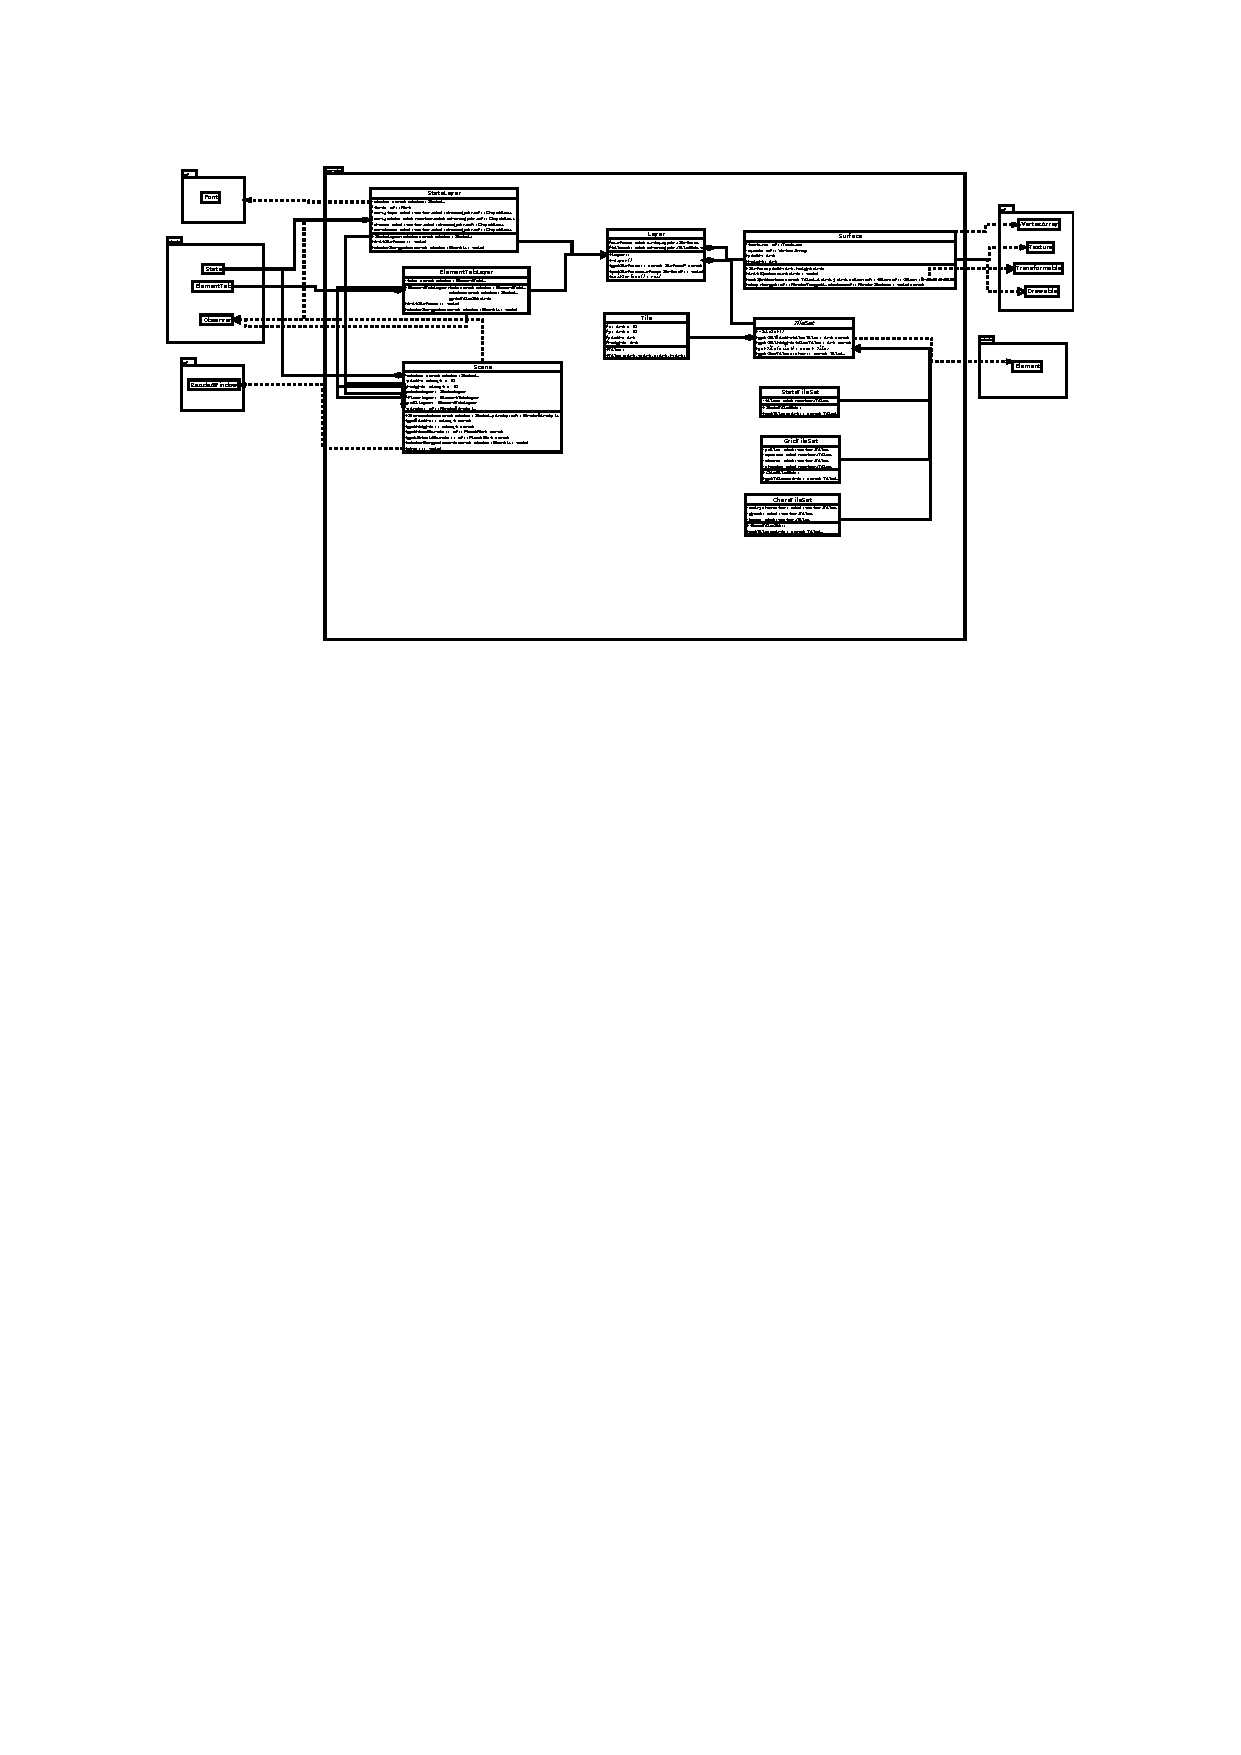
\includegraphics[width=0.9\paperheight]{render.pdf}
\caption{\label{uml:render}Diagramme des classes de rendu.} 
\end{figure}
\end{landscape}

\clearpage
\section{Règles de changement d'états et moteur de jeu}

\subsection{Changements extérieurs}

Nous avons des changements liés à des facteurs extérieurs, notamment avec la souris : 
- Une pression avec la souris sur le bouton "déplacement" (sur la droite de l'écran) affiche les possibilités de déplacement pour le personnage principal (les cases prennent une couleur verte)
- Une pression sur l'une de ces cases (donc uniquement après avoir pressé le bouton "déplacement") provoque le déplacement du personnage sur la case sélectionné.
- Lorsqu'un monstre se trouve sur une case adjacente de celle sur laquelle se trouve le personnage principal (pas les cases en diagonale), le joueur peut presser le bouton attaque pour infliger des dégâts au monstre, après plusieurs attaques, les pv de celui-ci tombent à 0 et le monstre disparaît de l'affichage.

\subsection{Changements autonomes}

Certains changements sont appliquées à chaque création ou mise à jour d'un état :
- Si le joueur se déplace sur une case qui se trouve à côté d'un monstre, alors il ne peut plus se déplacer avant la fin du combat (la mort du monstre), une fois le monstre vaincu et disparu, le personnage peut à nouveau se déplacer.
- Le joueur ne peut pas se déplacer sur des cases de type "mur"
- Les pv d'un monstre attaqué sont modifiés et s'ils arrivent à 0, le monstre disparaît de l'affichage.

\subsection{Conception logiciel}

Le diagramme des classes pour notre moteur de jeu est visible sur la page suivante. Celui-ci s'appuie sur différentes classes de type Command et a pour but l’exécution, dans un certain ordre, de différents types de commandes extérieures sur l'état du jeu.
\bigbreak
Classe Command et ses classes filles :
Chacune de ces classe vise à représenter un certain type de commande qui changera d'une manière ou d'une autre l'état de notre jeu, il est à noter que ce n'est pas dans ces classes que se déroule la gestion des entrées utilisateurs (appui sur une touche du clavier, de la souris ..).
On à également défini un type CommandTypeId pour identifier précisément la classe de n'importe quelle instance d'une commande.
Voici une description des différentes classes de commandes qui se trouvent actuellement dans notre diagramme des classes :
- MoveCommand, il s'agit de la classe qui gère les déplacements de notre personnage.
- PathCommand, cette classe s'occupe d'illuminer en vert les cases sur lesquelles le joueur peut se déplacer (n'illumine donc pas les cases "mur").
- AttackCommand, permet d'attaquer un monstre se trouvant sur une case adjacente (pas les diagonales)
Il reste 2 classes pas encore implémentés :
- LoadCommand, permet de charger une carte à partir d'un fichier, pour l'instant nous n'avons qu'une seule carte qui est chargée dès le lancement du jeu donc elle n'est pas encore implémenté.
- HandleCollisionsCommand, gère les collisions si le personnage et le monstre se trouvent sur la même case.
\bigbreak
Classe engine :
Cette classe représente le cœur de notre moteur de jeu. L'attribut currentState stocke l'état du jeu et l'attribut currentCommands est une std::map qui stocke les commandes à exécuter.
Grâce au format std::map, on introduit une priorité entre les commandes, les clés représentent la priorité, et plus elles sont petites, plus la commande sera exécuté tôt dans la liste .
A chaque appel de la méthode update(), le moteur va appeler la méthode execute de chacune des commandes stockées dans currentCommands puis nettoyer la liste (retirer toutes les commandes).
\bigbreak
A noter que les events liés à des actions du joueur (appui sur le clavier, souris ...) sont pour l'instant traitées dans le main(), nous comptons déplacer toute cette partie dans une classe dédiée à cela dans le render.

\begin{landscape}
\begin{figure}[p]
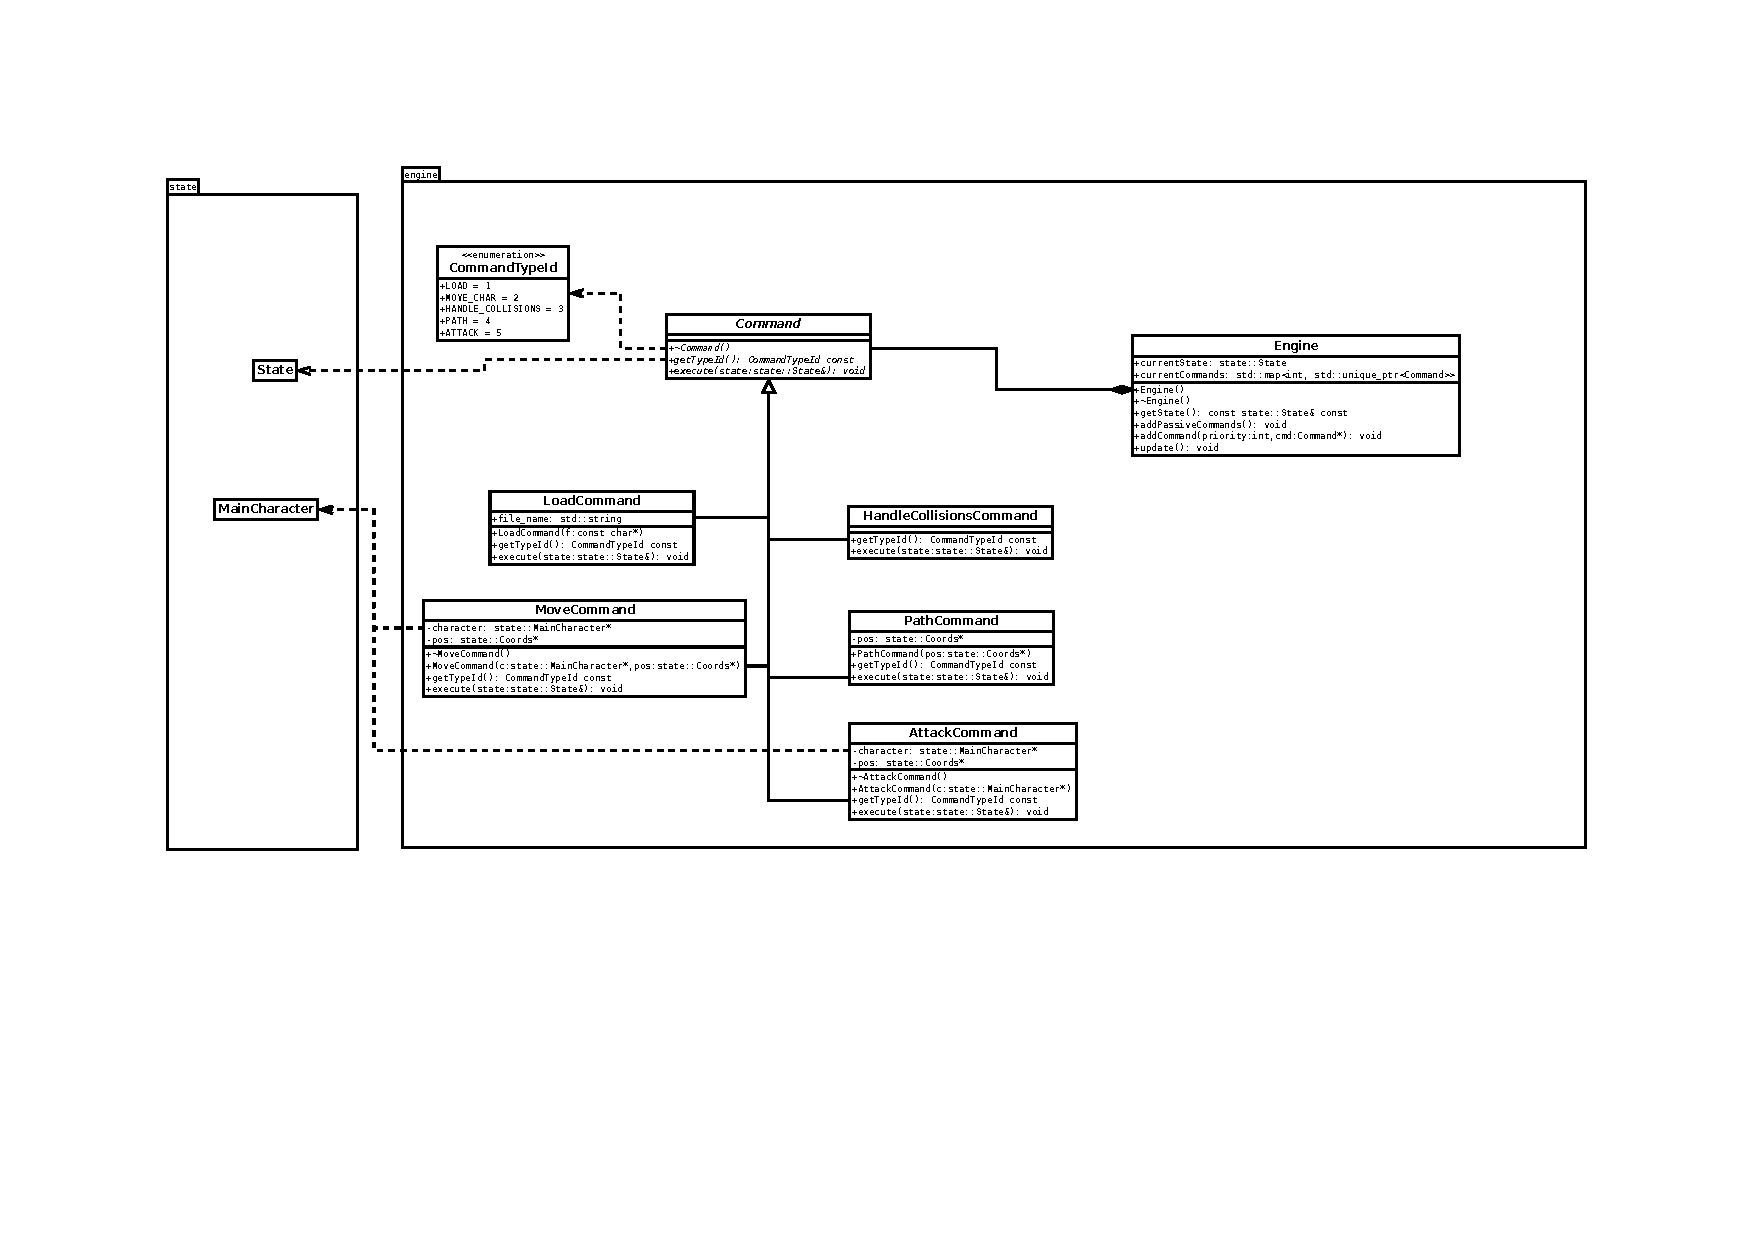
\includegraphics[width=0.9\paperheight]{engine.pdf}
\caption{\label{uml:engine}Diagramme des classes de moteur de jeu.} 
\end{figure}
\end{landscape}


\section{Intelligence Artificielle}

\subsection{Stratégies}

\subsubsection{Intelligence artificielle basée sur l'aléatoire}

Comme son nom l'indique, cette première intelligence artificielle est très basique et repose uniquement sur de l'aléatoire, à chaque nouveau tour, le personnage se déplace sur une case adjacente aléatoire

\subsubsection{Intelligence artificielle basée sur des heuristiques}

Cette intelligence artificielle est déjà plus développée que la précédente puisque cette fois-ci, les commandes possibles pour le personnage seront affectées d'un poids. Ce poids permettra d'effectuer des mouvements qui l'aideront à remplir son objectif : combattre et tuer un monstre disposé sur la map.

\subsubsection{Intelligence artificielle avancée}

L'IA avancée a pour but d'utiliser des algorithmes de résolution de problèmes à états finis vus en cours d'algorithmique. Nous choisissons donc d'utiliser un algorithme minmax pour obtenir une intelligence artificielle plus complexe, ceppendant, celle-ci s'avère aussi beaucoup plus gourmande en terme de calculs, c'est pourquoi, en cas de quantité  trop importante, on bascule sur l'IA heuristique afin de tout de me voir notre personnage bouger et réaliser son objectif.

\clearpage
\subsection{Conception logiciel}

Le diagramme des classes pour notre intelligence artificielle (ai.dia) est visible sur la page suivante.
\bigbreak
La classe AI est la classe mère de toutes les différentes intelligences artificielles que nous implémenterons dans différentes classes :
\bigbreak
- RandomAI : intelligence aléatoire, son fonctionnement est très peu complexe et cette classe ne nécessite qu'un attribut généré aléatoirement (ici randgen).
\bigbreak
-HeuristicAI : L'IA heuristique repose sur l'attribution de poids aux positions auxquelles le personnage peut accéder (les cases adjacentes), on définit donc l'attribut weight dans une classe Point qui importe les coordonnées (notée coord). 
La classe PathMap permet ensuite d'attribuer des poids aux points en fonction de la distance qui sépare le point de l'objectif du personnage (les monstres), plus la distance est petite, plus le poids est élevé.
\bigbreak
-AdvancedAI : Les algorithmes de notre IA avancée se divisent en 2 parties, la première partie consiste simplement à reprendre les algorithmes de l'IA heuristique pour s'assurer d'obtenir un comportement logique de notre IA même dans le cas où le minmax requiert trop de ressources/calculs. Pour savoir quand basculer d'une IA à l'autre, on utilise 2 variables définies dans la classe AdvancedAI que sont maxDepth, (pour la profondeur de l'arbre de recherche) et maxUpdates (pour le nombre d'étapes de recherche dans l'arbre).

Deuxièmement, une méthode minmax qui reprend l'algorithme vu en cours pour calculer les actions optimales à réaliser pour notre personnage en utilisant un système de score, nous nous sommes particulièrement inspirés d'un exemple sur un jeu de morpion.Cette méthode est récursive et va étudier toutes les cases autour de notre personnage.

Finalement, nous n'avons pas réussi à implémenter un minmax qui fonctionne, nous pensons que le problème est dû au trop grand nombre d'appels récursifs de la fonction minmax et au trop grand nombre de vérifications à effectuer aux alentours de notre personnage.

\begin{landscape}
\begin{figure}[p]
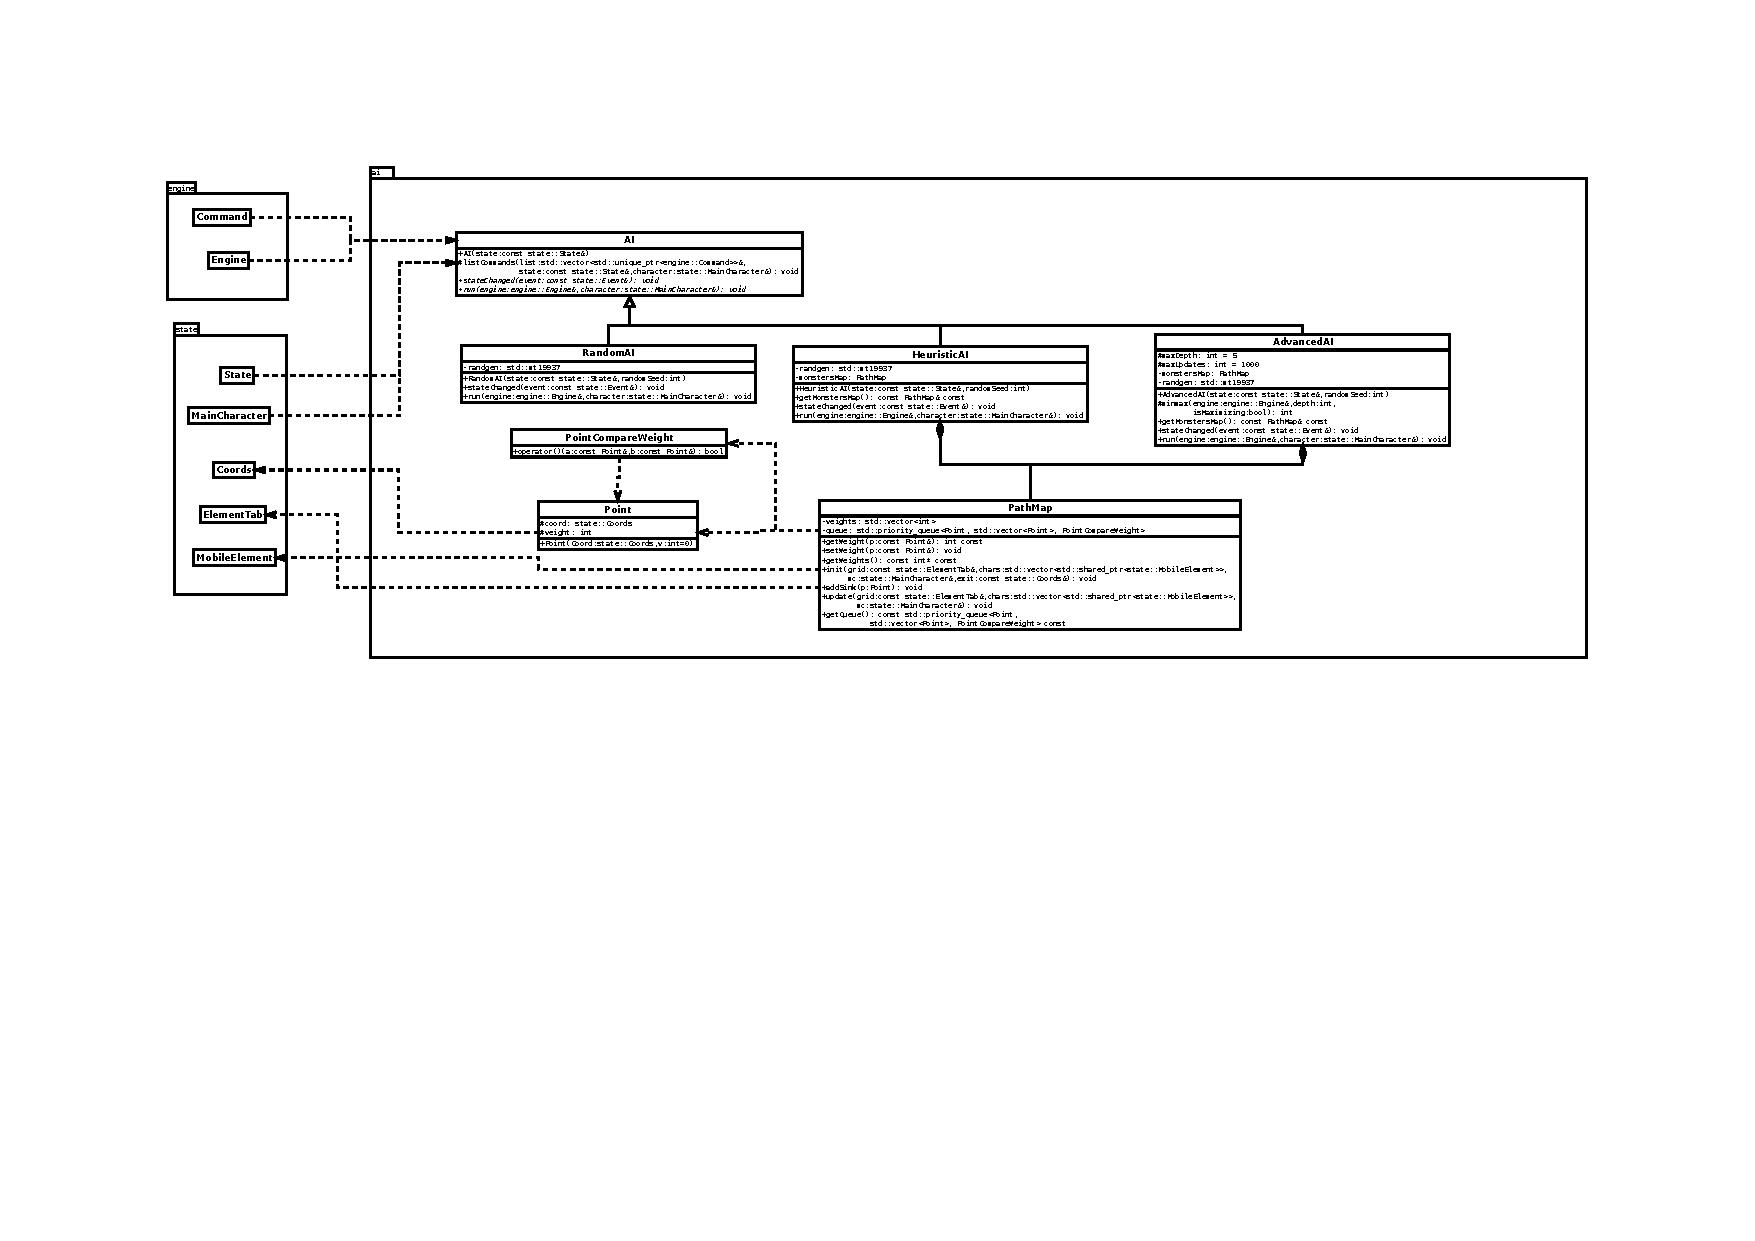
\includegraphics[width=0.9\paperheight]{ai.pdf}
\caption{\label{uml:ai}Diagramme des classes d'intelligence artificielle.} 
\end{figure}
\end{landscape}


%\section{Modularisation}
%\label{sec:module}
%
%\subsection{Organisation des modules}
%
%\clearpage
%\subsection{Conception logiciel}


%
%\begin{landscape}
%\begin{figure}[p]
%\includegraphics[width=0.9\paperheight]{module.pdf}
%\caption{\label{uml:module}Diagramme des classes pour la modularisation.} 
%\end{figure}
%\end{landscape}
 \addcontentsline{toc}{section}{Sources}
\section*{Sources}

\begin{itemize}
\item[Tiles :] DungeonTiles II \href{https://0x72.itch.io/dungeontileset-ii}{https://0x72.itch.io/dungeontileset-ii} par 0x72
\item[Font :] Pixel Font \href{https://devilsworkshop.itch.io/pixel-font}{https://devilsworkshop.itch.io/pixel-font


} par Ajay Karat | Devil's Work.shop
\end{itemize}

\end{document}
